% Energy figure (generated by efig_tex.py from efig.json, 2026-11-18 18:38 UTC)
\begin{figure*}[t]
  \centering
  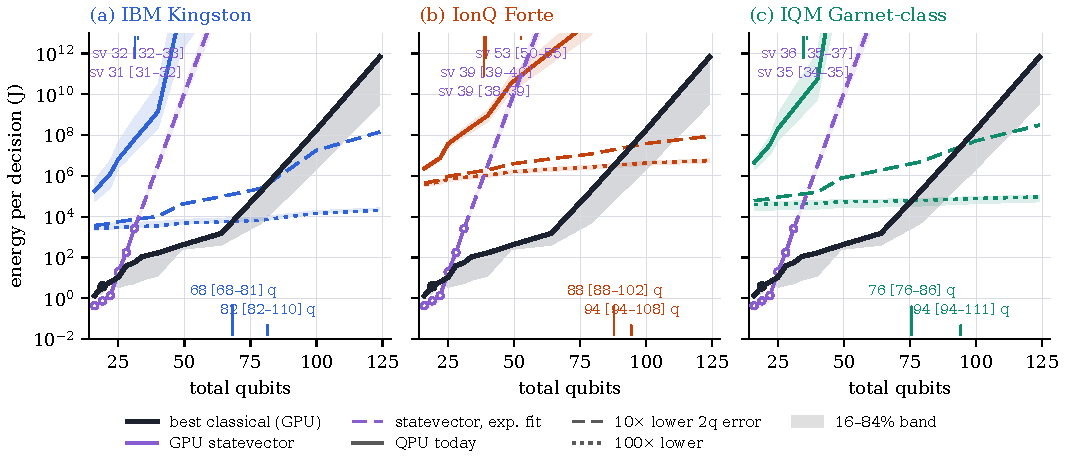
\includegraphics[width=\textwidth]{efig_log2.pdf}
  \caption{\textbf{Inference energy per decision: QPUs against the best classical method.} One image-choice decision of the CCG-structured post-selected circuit family (SVO-Probes standard test set), grown in qubits per wire, with depth $L=\mathrm{round}(\log_2 n_q)$. (a) Effective two-qubit gate error at which a QPU spends as much energy as the best classical method (circles) or as GPU statevector simulation only (triangles); horizontal lines mark each device\textquoteright s effective error today (solid) and 10$\times$ (dashed) and 100$\times$ (dotted) lower. A QPU wins below its curve; missing points: even an error-free QPU costs more. (b--d) Energy per decision (whole system) of each QPU at today\textquoteright s error and 10$\times$ and 100$\times$ lower two-qubit error, against the best classical method (black: cheapest of GPU statevector, exact tensor-network contraction, tensor-network sampler and MPS, path search amortised; filled markers measured, otherwise best-path upper bounds) and GPU statevector simulation (purple; dashed: exponential extrapolation). Shaded: 16th--84th percentile of 1000 Monte Carlo draws over workload, measurement, path-quality, interpolation, calibration, power and timing uncertainty (best classical: one-sided). Ticks mark crossovers with their intervals (bottom: below best classical; top, ``sv'': below statevector). Crossovers against the best classical method at 10$\times$ / 100$\times$ lower error: IBM Kingston 75 [75--102] / 66 [66--84] qubits; IonQ Forte 93 [93--109] / 88 [88--106] qubits; IQM Garnet-class 84 [84--105] / 73 [73--89] qubits; none at today's error up to 124 qubits. Against statevector only, at today's error: IBM Kingston 57 [50--70]; IonQ Forte 48 [45--50]; IQM Garnet-class 67 [58--82] qubits. Depths 6, 7 are interpolated from 4- and 8-layer circuits (preliminary). Setup and sources: Section~\ref{sec:energy-setup}.}
  \label{fig:energy}
\end{figure*}
